\chapter{Performance}
La metrica di confronto utilizzata nell'analisi degli algoritmi, è il tempo complessivo di creazione e risoluzione del modello. Ciascuna modalità di risoluzione viene applicata a diverse istanze di TSPlib, con un numero differente di nodi.  
\section{Performance variabilty}
Nel corso degli anni '90, gli ingegneri di CPLEX scoprirono che il tempo di risoluzione variasse significativamente tra UNIX e Windows. Con alcune istanze, le performance migliori si avevano su UNIX mentre con altre su Windows.\\
Il motivo di tale comportamento venne in seguito studiato e venne attribuito alla diversa scelta effettuata dai sistemi operativi nel decretare sull'ordine delle variabili su cui viene svolto l'albero decisionale.\\
Le scelte svolte inizialmente nella definizione dei primi nodi dell'albero, si ripercuotono sulla sua successiva evoluzione.\\
Proprio per questo motivo, su alcune istanze, UNIX riusciva a risolvere il problema in meno tempo rispetto a Windows, mentre su altre accadeva l'opposto.\\
Da questi studi, evinse che il Branch and Cut è un sistema caotico e che quindi piccole variazioni delle condizioni iniziali generano grandi differenze nei risultati finali.\\
Per questo motivo, i successi algoritmi sono stati studiati al variare di alcune condizioni iniziali:
\begin{itemize}
\item{\textbf{Random Seed}\\
Nel momento in cui CPLEX nota che diverse variabili frazionarie hanno lo stesso valore, il risolutore sceglie casualmente su quale di queste applicare il Branch.\\
La sequenza di numeri pseudo-casuali viene definita a partire dal random seed (vedi Sezione \ref{param}).}
\item{\textbf{Gap}\\
intervallo tra il valore della migliore funzione obiettivo intera e il valore della funzione di costo del miglior nodo rimanente (vedi Sezione \ref{param}).}
\item{\textbf{Node limit}\\
massimo numero di nodi risolti prima che l'algoritmo termini senza raggiungere l'ottimalità (vedi Sezione \ref{param}).}
\item{\textbf{Populate limit}
massimo numero di soluzioni MIP generata per il pool di soluzioni durante ogni chiamata della procedura di popolazione (vedi Sezione \ref{param}).}
\end{itemize}
La variazione del primo di questi parametri permette di mdificare il tempo di risoluzione non modficando la sua ottimalità. La variazione degli altri parametri permette di ottenere una soluzione meta-euristica, un'approssimazione più lasca.
 
\section{Analisi tabulare}
Un metodo non molto efficiente per lo studio delle performance dei vari algoritmi sviluppati, utilizza una struttura tabulare in cui viene inserita una riga per ogni istanza del problema.\\ Inoltre vengono riportati i tempi di risoluzione di ogni algoritmi su ogni grafo analizzato. Nell'ultima riga per ciascun algoritmo viene riportata la media geometrica dei suoi tempi di esecuzione (vedi esempio in Tabella \ref{result_table}).\\
Solitamente viene impostato un TIME LIMIT uguale per tutti gli algoritmi. Questo rappresenta nella tabella il valore del tempo di esecuzione per un algoritmo che ha impiegato un ammontare di tempo maggiore o uguale a TIME LIMIT.
Spesso viene dato più al TIME LIMIT, inserendolo nella tabella con valore 10 volte più grande.\\ La debolezza di tale calcolo delle performance risiede nel fatto che non semre la media descrive  l'efficienza di un soluzione. Infatti non influisce unicamente il tempo di risoluzione del modello ma anche quello necessario alla sua creazione. 

\begin{table}[h]
\centering
\begin{tabular}{|c|c|c|c|}
\multicolumn{1}{c}{\textbf{Istanza}} & \multicolumn{1}{c}{\textbf{Sequential}} & \multicolumn{1}{c}{\textbf{Flow}} &
\multicolumn{1}{c}{\textbf{Loop}}\\
\hline
\textbf{att48} & {212.3} & {12.5} & {4.3}\\
\hline
{\textbf{...}} & {...} & {...} & {...}\\
\hline
\textbf{a280} & {3200} & {2500.8} & {1300.5}\\
\hline
\hline
\multicolumn{1}{c}{} & \multicolumn{1}{c}{2120.3} & \multicolumn{1}{c}{1800.3}& \multicolumn{1}{c}{1000.4}\\
\end{tabular}
\caption{\footnotesize{Tabella di performance con TIMELIMIT=3200.}}\label{result_table}
\end{table}

\section{Performance profiling}
Questo metodo prevede la classificazione dei tempi di esecuzione degli algoritmi in base al numero percentuale di successi rispetto a un fattore (ratio) di moltiplicativo del tempo di esecuzione (vedi Figura \ref{perf_profile}).\\
L'andamento del performance profile di un algoritmo è monotono crescente. Il valore assunto per ogni ratio dagli algoritmi all'interno del grafico è la percentuale del numero di istanze che l'algoritmo risolve con quel fattore rispetto all'ottimo in quel caso.\\
Spesso questi grafici vengono rappresentati in scala logaritmica per notare al meglio le differenze ed avere una migliore raffigurazione da poter analizzare visivamente.

\begin{figure}[h] 
\begin{center} 
  % Requires \usepackage{graphicx} 
  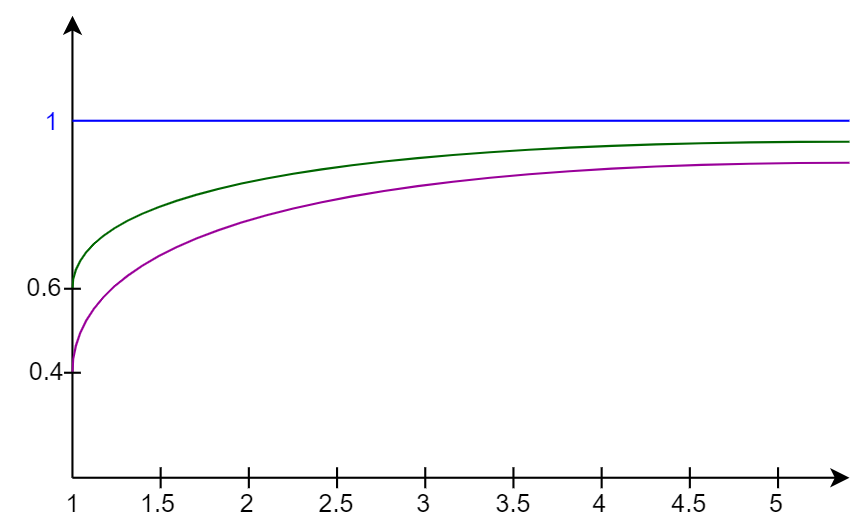
\includegraphics[scale=0.4]{Images/perf_profile}\\ 
  \caption{\footnotesize{Performance profile di due algoritmi.}}
  \label{perf_profile} 
\end{center} 
\end{figure}

Per creare il performance profile degli algoritmi implementati, è stato utilizzato il programma python riportato nella Sezione \ref{perf_profile_py}. 

\section{Analisi degli algoritmi sviluppati}
